
This work introduces a unified 3D frame element
library for OpenSees. 
The library will contain 6 elements, 4 cross
section models, and 4 geometric transformations as detailed below. 
All cross section models support shear deformations and at least one
warping mode, and should work seamlessly with all 6 elements whether or not they take such deformations into account.

This library addresses the following shortcomings in the existing
OpenSees offerings:

\begin{itemize}
\tightlist
\item
  No geometrically exact elements
\item
  Current elements do not handle distributed mass consistently
\item
  Cross section library is disjoint
\item
  Higher-order section kinematics are not handled consistently (e.g.
  Wagner strains)
\item
  Inconsistent treatment of asymmetric sections
\item
  Geometric transformations do not support shear or multi-node frame
  elements
\item
  Idiosyncrasies and inefficiencies in the corotational transformation
\end{itemize}

\clearpage
\subsection{Key Equations}
\RepeatEquation{eq:trace-map}

\begin{itemize}
    % \item \textbf{Trace State}
    %     Trace Strains:
    %     \RepeatEquation{eq:def-gam-kap}
    \item Element
        \begin{description}
            \item[$\circ$ Exact] \RepeatEquation{eq:finite-alignment-field}
            \item[$\circ$ Linear]
            \RepeatEquation{eq:trace-lift-linear}
        \end{description}
    \item Transform 
        \begin{equation}
        \overset{(1) \textbf{ Parameterization }}{
        \begin{Bmatrix}
        \mathtt{None} \\
        \mathtt{Incr} \\
        \mathtt{Init} \\
        \end{Bmatrix}
        }
        \times
        \overset{
        (2) \textbf{ Isometry}}{
        \begin{Bmatrix}
        \mathtt{None}  \\
        \mathtt{SFIN} \\
        \mathtt{Axis}  \\
        \end{Bmatrix}
        }
        \times
        \overset{
        (3) \textbf{ Interpolation }}{\begin{Bmatrix}
        \mathtt{None} \\
        \mathtt{Incr} \\ 
        \mathtt{Init} \\
        \end{Bmatrix}
        }
        \label{eq:chain}
        \end{equation}
    \item Section 
        \RepeatEquation{eq:saint-venant-stress}
        \RepeatEquation{eq:strain-tensor-decomp}
        \begin{description}
            \item[$\circ$ Wagner] \RepeatEquation{eq:wagner-gl-strain-pi}
            \item[$\circ$ Linear] \RepeatEquation{eq:linear-gl-strain-pi}
        \end{description}

    \item Saint~Venant, with \eqref{eq:trace-lift-linear}
     \begin{description}
        \item[Type 3]
          Trace Matrix:
          \RepeatEquation{eq:T0-inv}
          Fiber strain:
          \RepeatEquation{eq:eps-B-e}
          Resultants:
          \begin{description}
          \item[$\circ$ Petrov] 
          \RepeatEquation{eq:petrov-section}
          \item[$\circ$ Bubnov]
          \RepeatEquation{eq:bubnov-section}
          \end{description}
     \end{description}
\end{itemize}


\subsection{Element Library}\label{elements}
\begin{figure}[H]
    \centering
    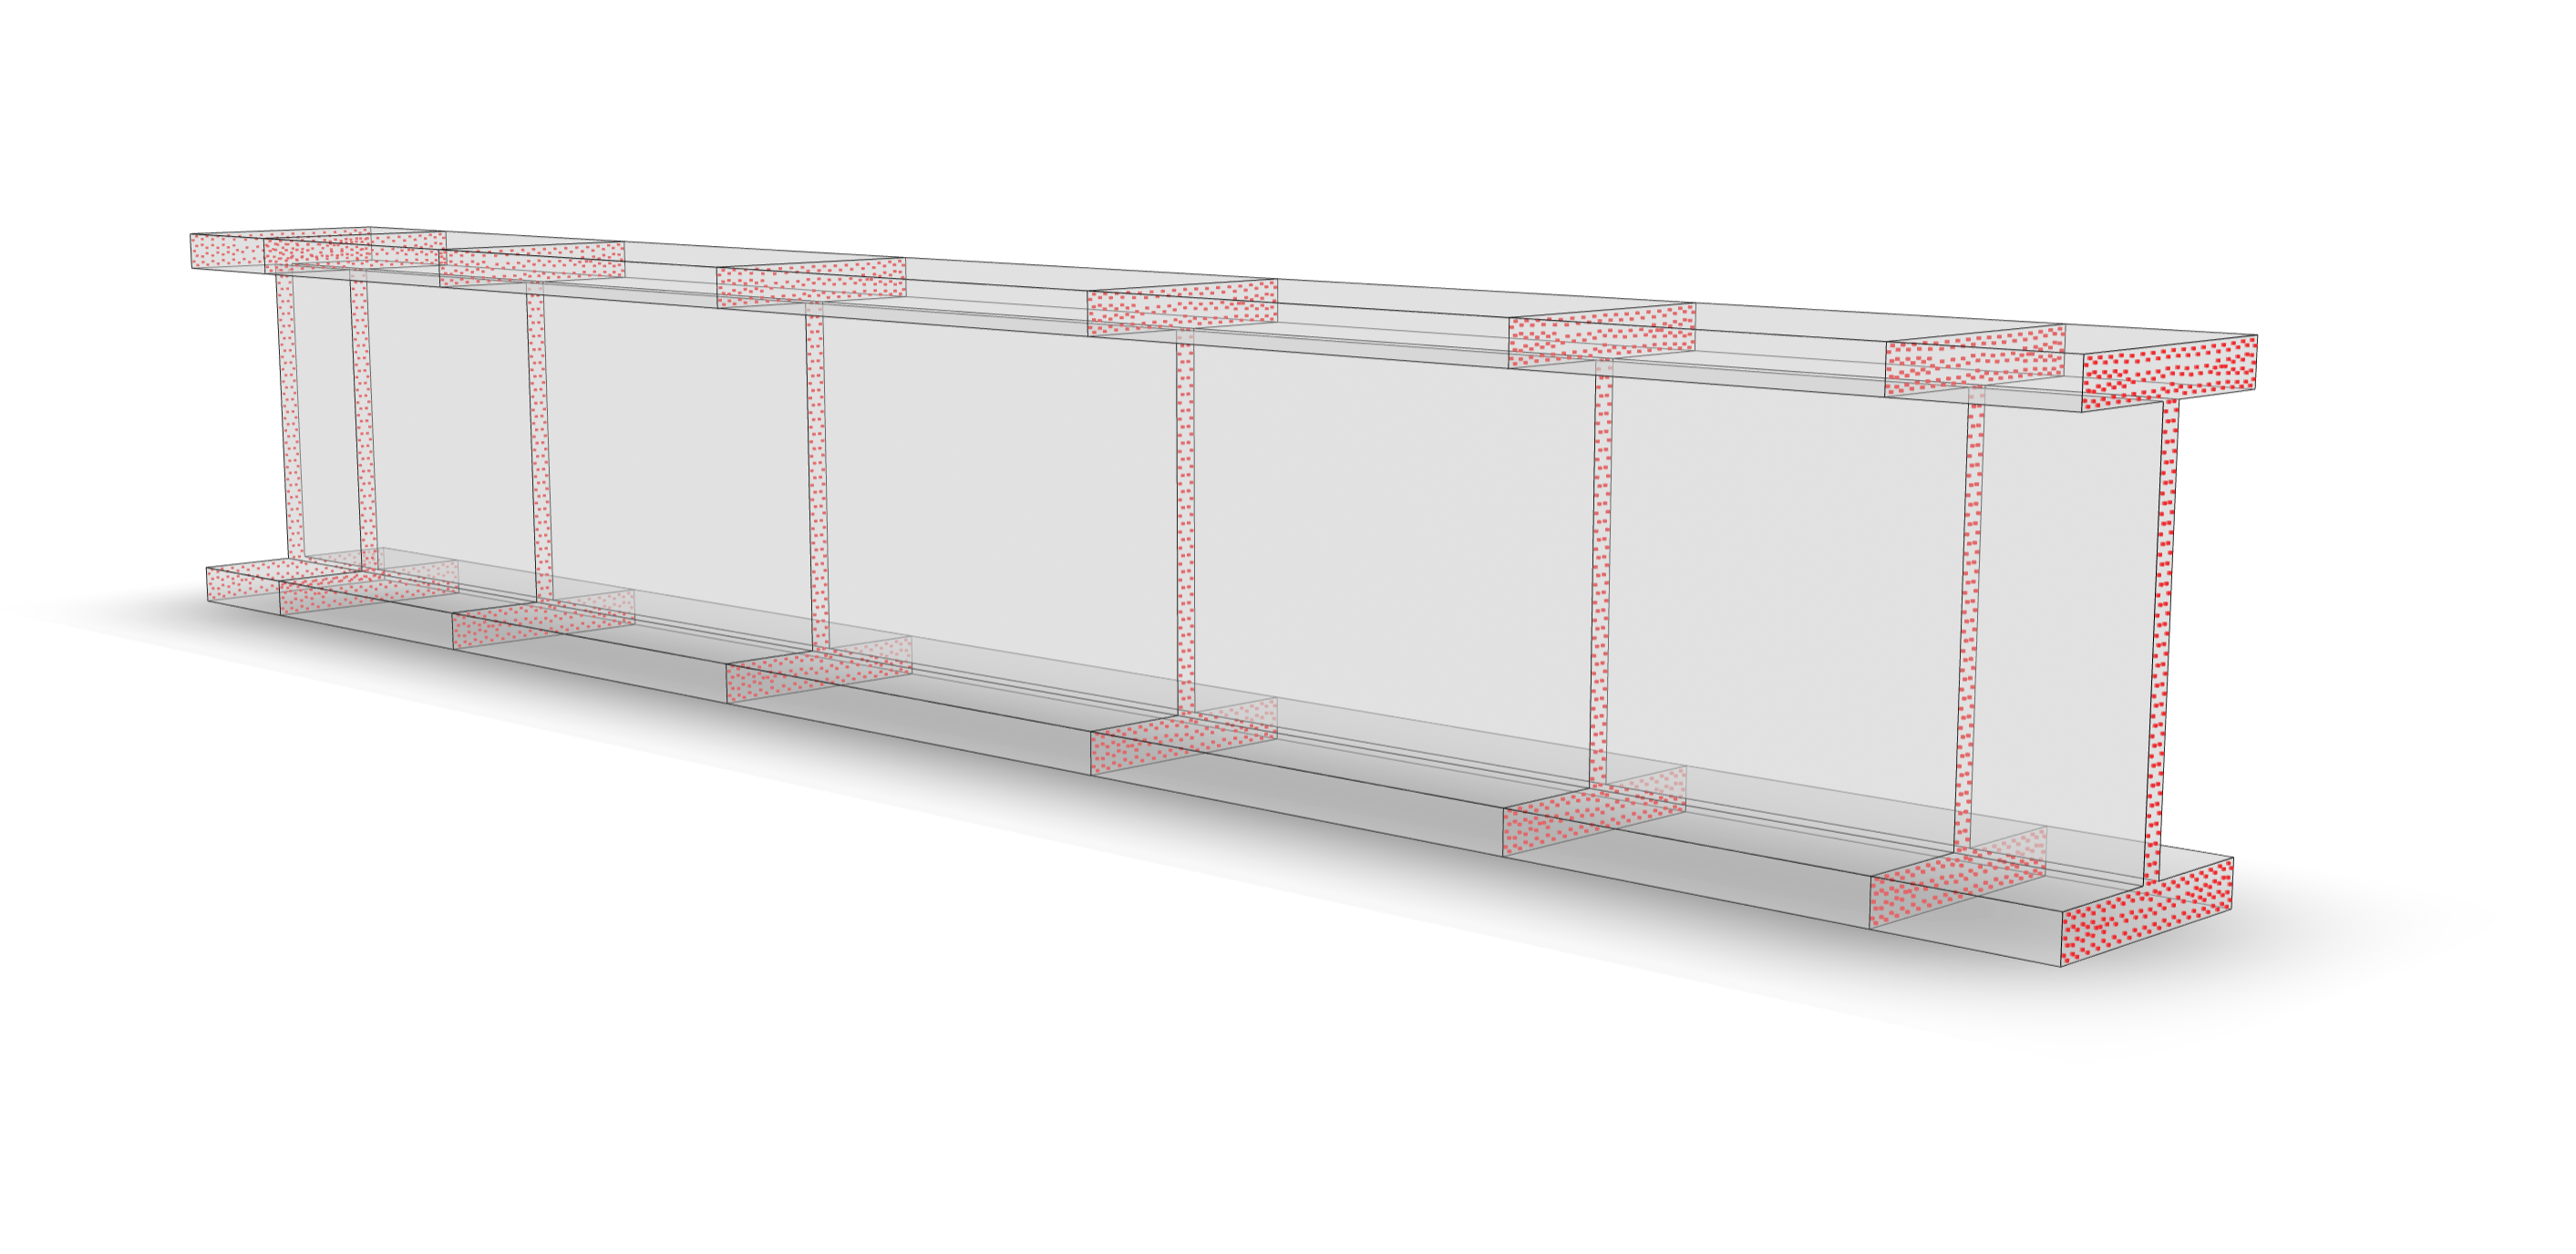
\includegraphics[width=0.75\linewidth]{Body/ForceFrame.png}
    \caption{Distributed-inelasticity frame element.}
    \label{fig:force-frame}
\end{figure}

There are six elements in the library, each supporting various options
for element kinematics. 
The element kinematic formulations are summarized in \cref{ch:frame-hierarchy} and are identified as
\gls{frame:exact}, \gls{frame:delta}, \gls{frame:axial} or \gls{frame:basic}. Each
of these kinematic formulations has a \gls{frame:shear} and \gls{frame:euler}
variant.

% \hypertarget{element-data}{%
% \subsection{Element Data}\label{element-data}}

All new frame elements will accept the following standard fields:

\begin{longtable}[]{@{}
  >{\raggedright\arraybackslash}p{(\columnwidth - 4\tabcolsep) * \real{0.1216}}
  >{\raggedright\arraybackslash}p{(\columnwidth - 4\tabcolsep) * \real{0.1622}}
  >{\raggedright\arraybackslash}p{(\columnwidth - 4\tabcolsep) * \real{0.7162}}@{}}
\toprule
\begin{minipage}[b]{\linewidth}\raggedright
Field
\end{minipage} & \begin{minipage}[b]{\linewidth}\raggedright
Type
\end{minipage} & \begin{minipage}[b]{\linewidth}\raggedright
Description
\end{minipage} \\
\midrule
\endhead
\texttt{transform} & Object & Reference to a pre-defined configuration
transformation \\
\texttt{section} & Object & Reference to a pre-defined cross section
model \\
\texttt{kinematics} & Flag & Optional variable specifying the kinematic
formulation of the element. \\
\texttt{shear} & Flag & Optional flag variable specifying the shear formulation. \\
\bottomrule
\end{longtable}

Note that by default elements will employ an appropriate integration
rule and the \texttt{section} field is used homogeneously. However, all
5 non-prismatic elements may alternatively be provided with an array of
section objects to account for inhomogeneity and an explicit integration
rule.

\paragraph{1. PrismFrame}
The \texttt{Prism} element is a standard linearly elastic prismatic
  frame. This element is ideal for modeling simple slender members that
  are not expected to exhibit inelastic response or experience
  excessively large deformations. Nonlinear effects from moderately
  large displacements can be accounted for using the \texttt{PDelta} or
  \texttt{Corotational} geometric transformations. Additionally, the
  \texttt{kinematics} option can be used to incorporate \(P-\delta\)
  effects with \texttt{Axial}  (\(P-\delta\)) element kinematics. Both \gls{frame:shear}
  and \gls{frame:euler} formulations are supported depending on the cross
  sectional properties supplied. This model is inherently elastic. If an
  inelastic section is supplied through the \texttt{section} argument,
  resultant stresses and stiffness are obtained by linearizing about the
  strain-free state. The implementation of 3D \gls{frame:axial} element
  kinematics is novel and supports asymmetric sections.


\paragraph{2. ForceFrame}
  The \ForceFrame{} element is ideal for modeling inelasticity in
  frames. Both \gls{frame:shear} and \gls{frame:euler} formulations are
  supported with \gls{frame:basic} and \gls{frame:axial} (\(P-\delta\)) element kinematics. 
  
  This element is adapted from the \texttt{forceBeamColumn} and
  \texttt{forceBeamColumnCBDI} elements of OpenSees and
  \texttt{Dinel3dFrm\_EBwFF} from FEDEASLab. 
  \textcite{spacone1992beam} developed the formulation for the \gls{frame:basic}-\gls{frame:euler} model presented in \cref{sec:basic-euler} and Box~\ref{box:basic-euler}.
%
  Geometric nonlinearities were considered in 2D by \textcite{neuenhofer1997evaluation} who introduced the concept of \emph{curvature-based displacement interpolation} (CBID). 
  This was later extended to the 3D \gls{frame:axial}-\gls{frame:euler} theory (Box~\ref{box:axial-euler}) by \cite{desouza2000forcebased}.
%
  The method was extended to the \gls{frame:basic}-\gls{frame:shear} theory through the work of \cite{taylor2003mixed,saritas2004modeling,saritas2009frame}.
%
  The CBDI technique was extended to the \gls{frame:axial}-\gls{frame:shear} theory of \cref{sec:axial-shear}  by \cite{jar}


\paragraph{3. CubicFrame}
  The \texttt{Cubic} element fits displacements to a cubic polynomial
  inside a 2-node basic system with optional shearing deformations. This
  element requires internal iterations in the presence of inelastic
  shear deformations. 
  The implementation of this element derives from
  the \texttt{Dinel3dFrm\_EBwDF} and \texttt{Dinel3dFrm\_TwDF*} elements
  of FEDEASLab.
  \begin{equation*}
      \mathbf{u}_a = \left(u_x,\, u_y,\, u_z,\, 
                           u_x',\, u_y',\, u_z',\, 
                           \alpha
                    \right)
  \end{equation*}


\paragraph{4. ExactFrame}
  The \ExactFrame{} element is a \(C^0\) displacement formulation of
  the exact shear-deformable element kinematics. 
  This element is ideal
  for modeling large elastic deformations. Reduced integration must be
  used to avoid shear locking, and consequently a combination of \(h\)
  and \(p\) refinement is required in order to adequately capture
  inelasticity.
  \begin{equation*}
      d\mathbf{u}_a = \left(u_x,\, u_y,\, u_z,\, 
                           \omega_x,\, \omega_y,\, \omega_z,\, 
                           \alpha
                    \right)
  \end{equation*}

% \subsection{Euler}
%   The \gls{frame:euler} element is a straightforward \(C^1\) displacement
%   formulation. Computations are performed in a local system.
%   \gls{frame:basic} and \gls{frame:axial} element kinematics are supported
%   with arbitrarily many nodes. The implementation of this element is not
%   derived from a preexisting element of OpenSees or FEDEASLab.

% \subsection{Shear}
%   The \gls{frame:shear} element is a straightforward \(C^0\) displacement
%   formulation. Computations are performed in a local system.
%   \gls{frame:basic} and \gls{frame:axial} element kinematics are supported.
%   Reduced integration must be used for this element to avoid shear
%   locking, and consequently a combination of \(h\) and \(p\) refinement
%   is required in order to adequately capture inelasticity.


\subsection{Transformation Library}\label{sec:transformation-types}

Elements are grouped into three types based on their geometric nature:

\begin{itemize}
\tightlist
\item
  \textbf{Type I} elements are formulated in a basic system and can only
  be connected with 2 nodes. Valid geometric transformations for these
  elements include \texttt{Linear}, \texttt{PDelta}, and
  \texttt{Corotational}.
\item
  \textbf{Type II} elements are formulated in a local system and can be
  connected with an arbitrary number of nodes. Valid geometric
  transformations for these elements include \texttt{Linear} and
  \texttt{Corotational}.
\item
  \textbf{Type III} elements are formulated in the global system using
  exact kinematics.
\end{itemize}

\subsection{Section Library}


\subsubsection*{Elastic}
\inputdraft{Body/Section/A_Constants}

\subsubsection*{AxialFiber}

\subsubsection*{ShearFiber}


\subsection{Sensitivity}
\cite{al-aukaily2019corotational}

\subsection{Summary}

\begin{longtable}[]{@{}
  >{\raggedright\arraybackslash}p{(\columnwidth - 10\tabcolsep) * \real{0.1978}}
  >{\raggedright\arraybackslash}p{(\columnwidth - 10\tabcolsep) * \real{0.1538}}
  >{\raggedright\arraybackslash}p{(\columnwidth - 10\tabcolsep) * \real{0.1538}}
  >{\raggedright\arraybackslash}p{(\columnwidth - 10\tabcolsep) * \real{0.1319}}
  >{\raggedright\arraybackslash}p{(\columnwidth - 10\tabcolsep) * \real{0.1429}}
  >{\raggedright\arraybackslash}p{(\columnwidth - 10\tabcolsep) * \real{0.2198}}@{}}
\toprule
\begin{minipage}[b]{\linewidth}\raggedright
Element Name
\end{minipage} & \begin{minipage}[b]{\linewidth}\raggedright
Shear
\end{minipage} & \begin{minipage}[b]{\linewidth}\raggedright
Euler
\end{minipage} & \begin{minipage}[b]{\linewidth}\raggedright
Transforms
\end{minipage} & \begin{minipage}[b]{\linewidth}\raggedright
Material
\end{minipage} & \begin{minipage}[b]{\linewidth}\raggedright
Interpolation
\end{minipage} \\
\midrule
\endhead
\texttt{Prism} & Basic, Axial & Basic, Axial & Type I & - & - \\
\ForceFrame & Basic, Axial & Basic, Axial & Type I & Section & - \\
\texttt{Cubic} (Displ.) & Basic & Basic & Type I & Section &
Cubic/Quadratic \\
\texttt{Mixed} & Basic, Axial & Basic, Axial & Type I & Section & - \\
\texttt{Euler} (Displ.) & - & Basic, Delta & Type II & Section & Hermite
(\(C^1\)) \\
\texttt{Shear} (Displ.) & Basic, Delta & - & Type II & Section &
Lagrange (\(C^0\)) \\
\texttt{Exact} (Displ.) & Exact & - & Type III & Section & Lagrange
(\(C^0\)) \\
\bottomrule
\end{longtable}
